\section{Design}
\label{sec:design}

\sys{} defines artifacts and rules, not a protocol stack.
Figure~\ref{fig:flow} shows how the artifacts ride on an A2A task.
Everything below is normative in the specification. We give its essential
content here and cite rule identifiers (\eg R-4) so readers can find the
full text.

\begin{figure}[t]
  \centering
  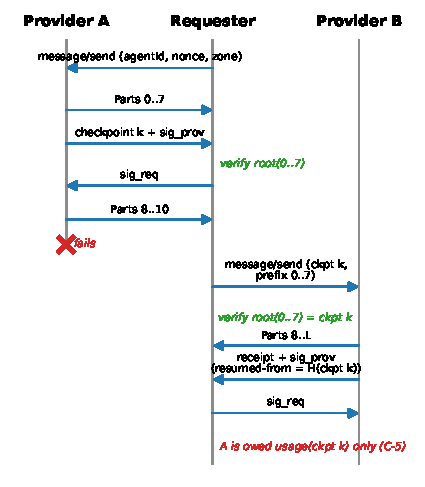
\includegraphics[width=\columnwidth]{figs/flow}
  \caption{A \sys{} task over A2A. Provider~A proposes checkpoints and the
  requester countersigns each one after recomputing the transcript root.
  When A fails, the requester resumes on Provider~B from the last
  countersigned checkpoint. B verifies the replayed prefix before it
  continues. B's work ends in a dual-signed receipt that names the
  checkpoint it resumed from. A is owed only the usage in that checkpoint
  (C-5).}
  \label{fig:flow}
\end{figure}

\subsection{Identity and encoding}
An agent is an Ed25519~\cite{rfc8032} public key (its AgentID). Every
artifact is a map in deterministic CBOR~\cite{rfc8949}. Each signature
covers a role-tagged signing input, $\mathit{enc}([\mathit{tag},
\mathit{role}, \mathit{core}])$, where the tag is \eg\texttt{"MAPReceipt"},
and the signature is carried either detached or in COSE\_Sign1~\cite{rfc9052}.
One invariant runs through all verification: a verifier checks signatures
over the bytes it \emph{received}, never over a re-serialization of
decoded values. That rules out a class of malleability bugs in which two
encodings of ``the same'' object verify differently. \sys{} fixes one
algorithm suite (Ed25519 and SHA-256) and negotiates nothing.

\subsection{Dual-signed execution receipts}
\label{sec:receipts}
A receipt's signed core names the task, the requester, the provider, the
capability, the start and end times, the outcome and the cumulative usage.
It optionally adds a rating, a voucher digest, the transcript root, the
data-sensitivity zone, and the checkpoint the task resumed from. Over A2A,
the provider proposes the receipt when the task reaches a terminal state,
and the requester countersigns it. The requester countersigns only if the
usage is within its own tolerance of what it observed; the tolerance is
local policy.

A receipt is \emph{admissible} evidence only if it passes four rules:
\begin{description}
\item[R-1] Each present signature verifies over the received bytes, and
  its signer is exactly the party named in the core.
\item[R-2] The requester and provider differ.
\item[R-3] \texttt{started} $\le$ \texttt{ended}, and \texttt{ended} is
  not in the evaluator's future beyond a skew bound (default 120\,s).
\item[R-4] Only a receipt signed by \emph{both} parties can be positive
  evidence. A requester-only receipt can only be negative (failed,
  timed out or disputed). A provider-only receipt counts for nothing.
\end{description}
R-4 is what makes evidence \emph{mutual}. A provider cannot mint praise
for itself, and a requester's complaint is attributable to that requester.
A provider that refuses to countersign its own failures (``selective
countersigning'') cannot suppress them, because the requester files a
unilateral negative receipt instead.

R-4 does \emph{not} stop a Sybil ring. The attacker there holds both
keys, so every receipt is genuinely dual-signed. Issuer weighting
(\S\ref{sec:trust}) is what closes it.

\subsection{Observer-local trust}
\label{sec:trust}
\paragraph{Rebuild rule.}
Trust is a \emph{projection}: derived data that any observer can
recompute from its receipt store. The rules:
\begin{itemize}
\item \textbf{T-1.} Rebuilding from the store must reproduce any
  incrementally maintained projection exactly. Decay uses the receipt's
  \texttt{ended} time, never the ingestion time, so arrival order does not
  matter.
\item \textbf{T-2.} R-1 to R-4 are part of the projection's
  \emph{apply} step, shared by incremental ingestion and by rebuild.
  Neither path can skip them.
\end{itemize}
We found T-2 the hard way. The first implementation checked the
dual-signature gate only on ingestion, so a rebuild silently admitted
unilateral positive receipts. An earlier review exploited exactly that
gap. It ran as AI-model sessions with no access to the implementation work
(Acknowledgments).

\paragraph{Scoring.}
The recommended score is Beta reputation~\cite{josang2002beta}. For each
admissible receipt $r$ about subject $s$ and capability $c$, let
$w(r) = \mathit{iw}(r)\cdot\lambda^{\Delta t}$, with decay
$\lambda = 0.98$ per day. Positive outcomes add $w(r)$ to $\alpha_{sc}$,
and failures add it to $\beta_{sc}$. The score is
$\alpha/(\alpha+\beta)$ under a $(1,1)$ prior. Its confidence
$\alpha+\beta$ is reported separately, because a score of 1.0 from one
receipt and a score of 0.97 from five hundred are different claims.
One issuer's total contribution to a subject is capped at 50 units, after
weighting.

\paragraph{Issuer weighting.}
\textbf{T-3} fixes the endpoints of the issuer weight $\mathit{iw}$: the
observer's own receipts weigh 1, and an issuer with no evidence
relationship to the observer weighs \emph{zero}. Zero, and not the
Beta prior's neutral 0.5, is the fix for receipt farming. In the ablation
where unknown issuers weigh 0.5, attackers win 72\% of honest requesters'
tasks under farming at $\alpha{=}0.2$, versus 2.5\% with weight 0
(\S\ref{sec:eval-trust}).

Between the endpoints, \sys{} compares three weightings:
\begin{itemize}
\item \textbf{W0} (self only) uses nothing but the observer's own
  receipts.
\item \textbf{W1} (direct agreement) weighs issuer $i$ by
  $a(o,i)=\max(0,\,1-2\cdot\mathrm{MAD}(o,i))$. The MAD is the mean
  absolute difference between $i$'s and the observer's per-provider
  success rates, taken over providers that both have rated at least 3
  times. At least 3 shared providers are required, or the weight is 0.
  This is the similarity weighting of PeerTrust and
  Credence~\cite{xiong2004peertrust,walsh2006credence}.
\item \textbf{W2} (propagation) is personalized
  PageRank~\cite{page1999pagerank}, in the spirit of
  EigenTrust~\cite{kamvar2003eigentrust}, over the row-normalized
  agreement graph of all issuers: 10 steps with restart 0.15 to the
  observer, and $\mathit{iw}(i)=\min(1,t_i/t_o)$.
\end{itemize}
The specification recommends \textbf{W1}. \S\ref{sec:eval-trust} explains
why this differs from our pre-registered choice.

\subsection{Countersigned checkpoints and resumption}
\label{sec:checkpoints}
\paragraph{Transcript.}
The provider's output Parts form a Merkle tree over SHA-256. A leaf is
$H(\mathtt{0x00}\,\|\,\mathit{enc}([\mathit{seq},\mathit{kind},
\mathit{content}]))$ and an interior node is
$H(\mathtt{0x01}\,\|\,l\,\|\,r)$. The domain separation rules out
leaf/interior confusion.

\paragraph{Checkpoints.}
A \texttt{CheckpointArtifact} signs a core with these fields:
\begin{itemize}
\item the task, requester and provider;
\item \texttt{through-seq};
\item the transcript root over Parts $0..\mathit{through\text{-}seq}$;
\item cumulative usage and the zone;
\item optionally, a voucher digest and a resumed-from digest.
\end{itemize}
The signing order is fixed:
\begin{itemize}
\item \textbf{C-1.} The provider signs first.
\item \textbf{C-2.} The requester countersigns only after recomputing the
  root from the Parts it actually received.
\item \textbf{C-3/C-4.} \texttt{through-seq} strictly increases between
  checkpoints, and usage never decreases.
\end{itemize}
A checkpoint with both signatures is a \emph{valid resumption point}.

\paragraph{Resumption.}
When a provider fails, the requester sends a successor the last valid
resumption point together with the transcript prefix it covers. The
successor recomputes the root and refuses to continue on any mismatch.
Its own receipt carries \texttt{resumed-from}, the digest of that
checkpoint. The providers need not know each other, and continuation need
not be deterministic across them: the seam is visible in the transcript.

\paragraph{Scope of resumption.}
The transcript holds only the Parts a provider delivered. Resuming from
it is complete only for tasks whose state \emph{is} their output, such as
streamed generation. A provider's hidden state is not in the transcript,
including tool results, scratchpads and working files. A successor also
cannot see external side effects its predecessor caused, such as a
payment or a write, so it may repeat them. \sys{} does not make such
effects idempotent. Tasks that have them need application-level
checkpoints or idempotency keys, which are outside this layer.

\paragraph{Billing bound.}
\textbf{C-5}: a failed provider is owed only the usage in its last
countersigned checkpoint. It is never owed a figure it claimed
afterwards. Overbilling is therefore bounded by one checkpoint interval
$c$. The default (C-6) depends on how countersignatures travel. It is
$c{=}8$ Parts when they return asynchronously while the task keeps
running, and $c{=}32$ when the provider pauses for each one. Both come
from the evaluation (\S\ref{sec:eval-checkpoint},
\S\ref{sec:eval-meter}).

\subsection{Evidence-bound metering}
\label{sec:metering}
\sys{} does not move money. Checkpoints and receipts may carry
\texttt{voucher-digest}, the hash of the payer-signed cumulative voucher
that covers the usage they record. This is a \emph{reverse} binding.
The rail's voucher format is untouched, yet anyone holding both artifacts
can prove they refer to the same delivery. A requester should not sign a
voucher beyond the price of its last countersigned checkpoint plus the
credit it deliberately extends (M-6). Pausing and resuming delivery are
left to the rail: MPP's session updates and x402's batch
settlement~\cite{mpp2026,x402v2}. Amounts are unsigned integers. A
negative amount therefore cannot be encoded, which removes a v1 bug in
which a negative payment moved funds backwards.

\subsection{Zones}
\label{sec:zones}
A task carries a data-sensitivity label $z\in\{0..3\}$, from local-only
to open. A counterparty's zone is the \emph{requester's} classification
of it (allowlisted, authenticated mesh peer, or ephemeral), never the
provider's own claim.
\begin{itemize}
\item \textbf{Z-1.} A zone-$z$ task may go only to a counterparty
  classified $\le z$.
\item \textbf{Z-2.} The label is inside the dual-signed checkpoint and
  receipt, so a provider cannot later deny the handling obligation it
  accepted.
\item \textbf{Z-3.} A label never widens along a resumption chain.
\end{itemize}
Zones make mishandling attributable, not impossible.

\subsection{Two-plane discovery}
\label{sec:discovery}
The \emph{stable plane} holds signed descriptors, which embed the
provider's signed A2A Agent Card (\S\ref{sec:binding}). They are
published into a Kademlia DHT under sharded capability keys
$K(\mathit{cap},s)$, with $s=\mathrm{SHA\text{-}256}(\mathit{AgentID})[0]$.
A querier samples a few random shards and merges the results. The DHT is
untrusted storage.
\begin{itemize}
\item \textbf{D-6.} The querier discards any record whose AgentID does not
  belong in the shard it was found under, and verifies every descriptor
  signature before shortlisting it.
\item \textbf{D-9.} Queriers should use $d{=}3$ disjoint-path lookups, in
  the style of S/Kademlia~\cite{baumgart2007skademlia}.
\end{itemize}
The \emph{volatile plane} (queue length, estimated latency) is pulled on
demand from the shortlist with a \texttt{StatusQuery}. It is not
carried in descriptors, because a cached value is stale when it matters
(\S\ref{sec:eval-discovery}).
